\hypertarget{moderne-blockverschluxfcsselungsverfahren}{%
\section{Moderne
Blockverschlüsselungsverfahren}\label{moderne-blockverschluxfcsselungsverfahren}}

\hypertarget{data-encryption-standard---des}{%
\subsection{Data Encryption Standard -
DES}\label{data-encryption-standard---des}}

\emph{Block size: 64}\\
\emph{Key size: 56 (+ 8 parity bits)}\\
\emph{Structure: Feistel network}\\
\emph{\# of Rounds: 16}

\hypertarget{feistel-network}{%
\subsubsection{Feistel Network}\label{feistel-network}}

\begin{figure}[H]
\centering
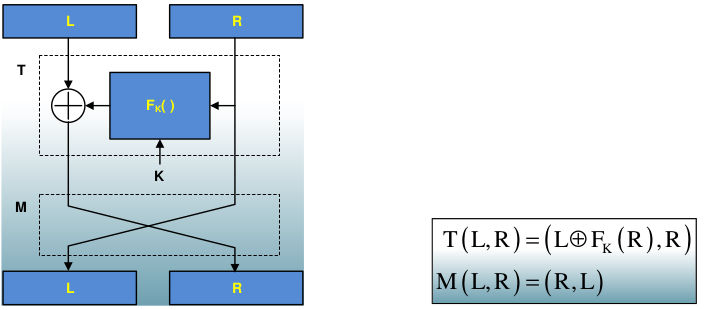
\includegraphics[width=1\textwidth]{figures/feistelNetwork.png}
\caption{Feistel Network}
\end{figure}

\begin{itemize}
\tightlist
\item
  Zuerst wird die Nachricht in die Hälften Rechts und Links aufgeteilt
\item
  Mit der rechten Hälfte passiert nichts. Sie wird nur zur linken Hälfte
  gemacht.
\item
  Die rechte Hälfte wird mit dem Rundenschlüssel (Fk) verschlüsselt und
  dann mit der linken Hälfte XOR verknüpft.
\item
  Unabhängig von Fk(R) kann dieselbe Feistel Struktur verwendet werden,
  um die Nachricht wieder zu entschlüsseln.
\end{itemize}

\hypertarget{des-ablauf}{
\subsubsection{DES Ablauf}\label{des-ablauf}}

\begin{figure}[H]
\centering
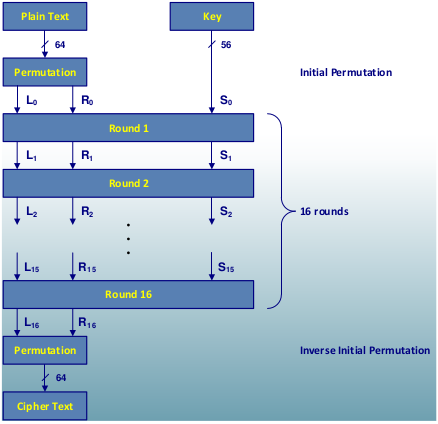
\includegraphics[width=0.5\textwidth]{figures/dataEncryptionStandard.png}
\caption{Feistel Network - Ablauf}
\end{figure}

\begin{itemize}
    \item Bevor der Algorithmus anfängt, werden die Eingangsbits zuerst noch permutiert (Initial Permutation)
    \item Jede Runde wird ein Feistel Netzwerk durchgeführt
    \item Es gibt ein Hauptschlüssel aus 56 bits
    \item In jeder Runde wird ein Rundenschlüssel aus dem Hauptschlüssel abgeleitet
    \item Am Schluss aller Runden werden die Bits ebenfalls nochmals permutiert.
\end{itemize}

\hypertarget{rundenschluxfcssel}{%
\subsubsection{Rundenschlüssel}\label{rundenschluxfcssel}}

\begin{itemize}
\tightlist
\item
  Der wird ebenfalls in eine linke und eine Rechte Hälfte geteilt
\item
  In jeder Runde werden die beiden Hälften zyklisch Bit-geschiftet
\item
  Aus den zur verfügungstehenden 56 Bits werden nach bekannten Regeln 48
  Bits ausgewählt, mit denen dann weitergearbeitet wird.
\end{itemize}

Das folgende Bild zeigt eine einzelne Runde im DES Ablauf.

\begin{figure}[H]
\centering
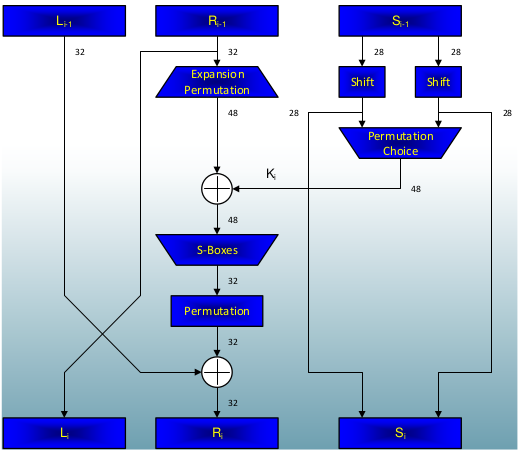
\includegraphics[width=0.7\textwidth]{figures/singleRoundDES.png}
\caption{Einzelne Runde DES}
\end{figure}

\hypertarget{mittlerer-ablauf}{%
\subsubsection{Mittlerer Ablauf}\label{mittlerer-ablauf}}

Wie in der Abbildung der einzelnen Runde im DES dargestellt wird, wird
die XOR Verknüpfung mit 48 Bits gemacht. Damit aus den 32 Bits von der
rechten Eingangshälfte 48 werden, wird eine Expansions Permutation
angewendet. Dies ist eine bekannte Regel, die aus den 32 Bits 48 macht.
Das folgende Bild ist ein Beispiel für eine solche Expansion Permutation
(muss nicht auswendig gelernt werden.)

\begin{figure}[H]
\centering
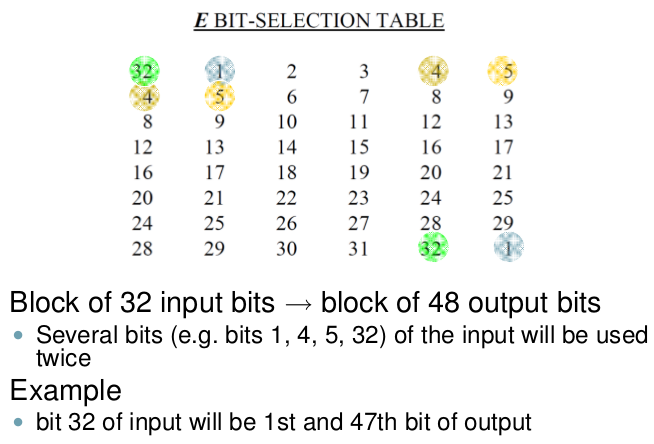
\includegraphics[width=0.5\textwidth]{figures/expansionPermutation.png}
\caption{Beispiel Expansion Permutation}
\end{figure}

\clearpage
\hypertarget{s-boxes-herzstuxfcck}{%
\subsubsection{S-Boxes (Herzstück)}\label{s-boxes-herzstuxfcck}}

\emph{Konfusion kommt nur vor, wenn in einem Algorithmus etwas
nicht-lineares steckt.}

\begin{itemize}
\tightlist
\item
  Insgesamt 8 S-Boxen
\item
  Jede S-Box hat 6 Bits am Eingang
\item
  Jede S-Box hat 4 Bits am Ausgang
\end{itemize}

\textbf{Vorgehen}: 
\begin{itemize}
    \item Man nehme von den 6 Bits das Bit ganz rechts und das ganz Links. Beide Bits zusammen ergibt eine Dezimalzahl, die Zeile.
    \item Man nehme die restlichen 4 Bits und bildet ebenfalls eine Dezimalzahl. Dies ergibt eine Zahl zwischen 0 und 15, also die Spalte.
    \item Die resultierende Zeile und Spalte ergibt eine neue Dezimalzahl zwischen 0 und 15, dies ergibt die 4 Bits vom Ausgang.
\end{itemize}

\begin{figure}[H]
\centering
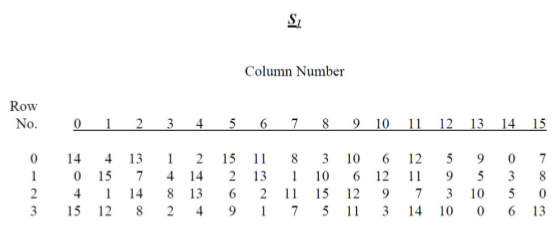
\includegraphics[width=0.7\textwidth]{figures/sBox1.png}
\caption{Beispiel für eine S-Box}
\end{figure}

\hypertarget{sicherheit}{%
\subsubsection{Sicherheit}\label{sicherheit}}

Key von 56 bits ist zu klein! \textbf{Bruteforce möglich!}.

\hypertarget{triple-des}{%
\subsection{Triple DES}\label{triple-des}}

\begin{itemize}
\tightlist
\item
  DES wird dreimal ausgeführt, jedoch zuerst chiffriert, dann
  dechiffriert und dann wieder chiffriert
\item
  Es ist möglich

  \begin{itemize}
  \tightlist
  \item
    drei verschiedene Keys zu wählen
  \item
    Key 1 und 3 gleich wählen, aber 2 unabhängig
  \item
    Alle drei Keys gleich wählen (kompatibel zu single DES)
  \end{itemize}
\item
  Zwei mal DES ist nicht sicher --\textgreater{}
  ``meet-in-the-middle-Attacke''
\end{itemize}

\begin{figure}[H]
\centering
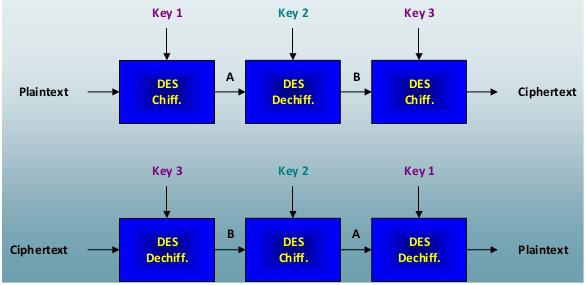
\includegraphics[width=0.8\textwidth]{figures/tripleDES.png}
\caption{Triple DES}
\end{figure}

\hypertarget{advanced-engryption-standard---aes}{%
\subsection{Advanced Engryption Standard -
AES}\label{advanced-engryption-standard---aes}}

\emph{Block size: 128}\\
\emph{Key size: 128/192/256}\\
\emph{\# of Rounds: 10/12/14}

\begin{itemize}
\tightlist
\item
  Man bekommt 128 Bits in Klartext
\item
  Die unterteilt man in 16 8 Bit Blöcke
\item
  Die 16 Blöcke legt man in eine 4x4 Matrix ab
\item
  Ergibt eine 4x4 Matrix mit 8 Bits pro Feld = 128 Bit, die
  \textbf{Zustandsmatrix}
\item
  Die Werte in den Feldern werden nicht als Dezimalzahl interpretiert,
  sondern als Element im endlichen Körper $GF(2^8)$ mit dem irreduzierbaren
  Polynom m(x) = $x^8+ x^4 + x^3 + x + 1$
\end{itemize}

\hypertarget{ablauf-aes}{%
\subsubsection{Ablauf AES}\label{ablauf-aes}}

Vier Arten von Operationen: - AddRoundKey - SubBytes - ShiftRows -
MixColumns (wird beim letzten Durchlauf weggelassen)

\begin{figure}[H]
\centering
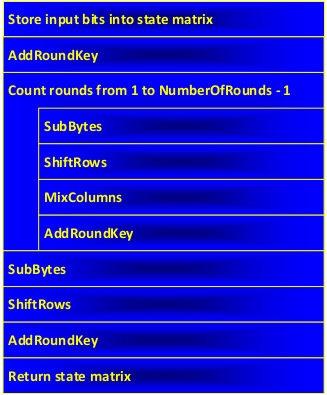
\includegraphics[width=0.4\textwidth]{figures/ablaufAES.png}
\caption{Ablauf AES}
\end{figure}

\hypertarget{addroundkey}{%
\subsubsection{AddRoundKey}\label{addroundkey}}

Sie nehmen einen Eintrag aus der Zustandsmatrix und einen Eintrag aus
der Rundenschlüsselmatrix und machen eine XOR Verknüpfung.

\hypertarget{subbytes}{%
\subsubsection{SubBytes}\label{subbytes}}

Substitution von Bytes. Die Bytes in der Zustandsmatrix werden anhand
einer Permutationstabelle durch neue Bytes ersetzt.

\begin{figure}[H]
\centering
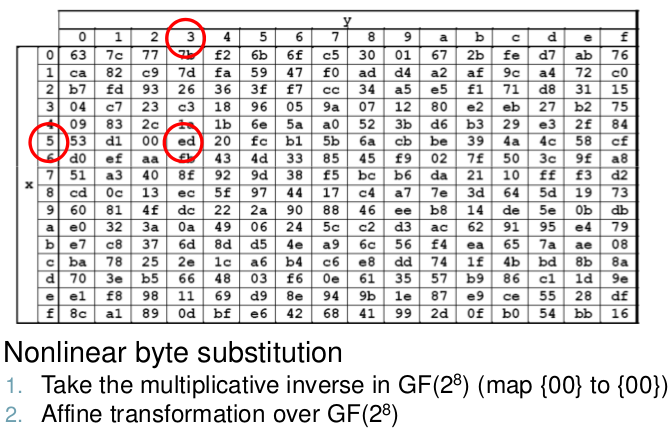
\includegraphics[width=0.7\textwidth]{figures/subBytesAES.png}
\caption{SubBytes AES}
\end{figure}

\hypertarget{shiftrows}{%
\subsubsection{ShiftRows}\label{shiftrows}}

Die Zeilen werden geshiftet. Die erste Zeile gar nicht, die zweite
zweimal, die dritte dreimal, die vierte viermal.

\begin{figure}[H]
\centering
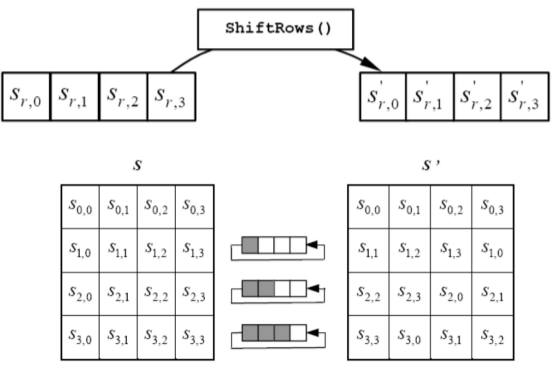
\includegraphics[width=0.6\textwidth]{figures/aesShiftRows.png}
\caption{Shift Rows AES}
\end{figure}

\hypertarget{mixcolumns}{%
\subsubsection{MixColumns}\label{mixcolumns}}

Eine Spalte der Zustandsmatrix wird auf eine neue Spalte der
Zustandsmatrix abgebildet. Dabei wird jede einzelne Spalte mit einer
definierten Matrix multipliziert. Dabei ist zu beachten, dass sich alle
Einträge im Raum $GF(2^8)$ befinden und mit Modulo $x^4+1$ multipliziert
werden.

\hypertarget{decryption}{%
\subsubsection{Decryption}\label{decryption}}

Alle Operationen haben eine invertierte Operation, die zum Entschlüsseln angewendet wird: $AddRoundKey \Leftrightarrow AddRoundKey - ShiftRows  \Leftrightarrow  InvShiftRows - SubBytes  \Leftrightarrow  InvSubBytes - MixColumns  \Leftrightarrow  InvMixColumns$

\hypertarget{international-data-encryption-algorithm---idea}{%
\subsection{International Data Encryption Algorithm -
IDEA}\label{international-data-encryption-algorithm---idea}}

\begin{itemize}
\tightlist
\item
  Long key:\\
  The 128-bit key gives a large margin of safety against cryptanalysis.
\item
  Confusion:\\
  Mixes three ``incompatible'' group operations so that no two
  successive operations are of the same type.
\item
  Diffusion:\\
  Provided for by the ``Multiply-Add (M-A) Box''
\item
  Encryption/Decryption Similarity:\\
  Encryption and decryption differ only in the key schedule used.
\item
  Scalable:\\
  Mini-versions (2-bit, 4-bit or 8-bit symbols) can be studied for
  possible weaknesses and analysis.
\item
  Transparency:\\
  No reliance on ``random-looking'' tables or ``mysterious'' S-boxes.
\item
  Easy to substitute for DES:\\
  Both have a plaintext and ciphertext block length of 64 bits.\\
  The userselected key is twice as long.
\item
  Fast in software and in hardware.
\item
  As much provable security as possible:\\
  For instance, ``perfect secrecy'' in one-round with a onetime key.
\end{itemize}

\hypertarget{operationen}{%
\subsubsection{Operationen}\label{operationen}}

Drei Operationen, die nicht miteinander verknüpft werden können. 
\begin{itemize}
    \item Bitweise XOR Verknüpfung
    \item Addition modulo $2^{16}$
    \item Mulitplikation mit modulo $2^{16}+1$ mit Zahlen, die nicht 0 sind.
\end{itemize}

\hypertarget{multiply-add-box}{%
\subsubsection{Multiply-Add Box}\label{multiply-add-box}}

Dies ist das Herzstück des IDEA. Jedes Output-Bit ist von jedem
einzelnen Input-Bit abhängig.

\begin{figure}[H]
\centering
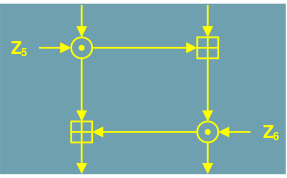
\includegraphics[width=0.5\textwidth]{figures/ideaMultiplyAddBox.png}
\caption{Multiply Add Box}
\end{figure}

\hypertarget{vorgehen}{%
\subsubsection{Vorgehen}\label{vorgehen}}

\begin{figure}[H]
\centering
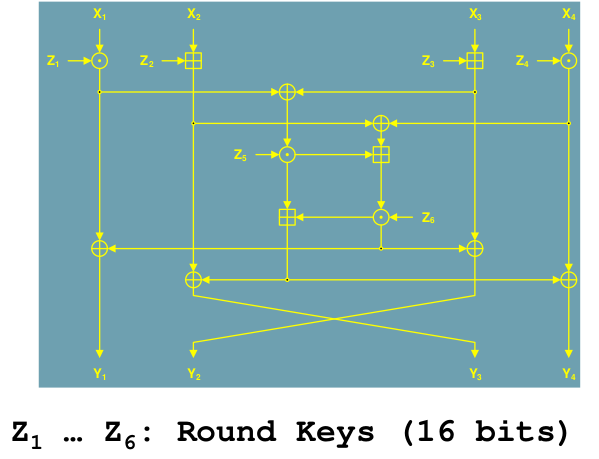
\includegraphics[width=0.5\textwidth]{figures/ideaAblauf.png}
\caption{Ablauf IDEA}
\end{figure}

In der letzten Runde werden die ersten Operationen nochmals ausgeführt.
Dies ist deshalb wichtig, weil man dann auch die Decryption mit
derselben Hardware machen kann.

\clearpage
